\chapter{Аналитическая часть}

В данном разделе будет рассмотрена задача коммивояжера и будут описаны алгоритмы её решения.

\section{Задача коммивояжера}

Цель задачи коммивояжера \cite{model} заключается в нахождении самого выгодного маршрута (кратчайшего, самого быстрого, наиболее дешевого), проходящего через все заданные точки (пункты, города) по одному разу.

Условия задачи должны содержать критерий выгодности маршрута (должен ли он быть максимально коротким, быстрым, дешевым или все вместе), а также исходные данные в виде матрицы затрат (расстояния, стоимости, времени) при перемещении между рассматриваемыми пунктами.

\subsection{Математическая модель}

Исходные условия можно представить в виде взвешенного графа - конечного множества вершин и множества ребер, соединяющих вершины. Вершины символизируют города, ребра - пути между городами, вес ребра - стоимость пути.

Рассмотрим взевешенный граф на рисунке \ref{img:graph}. Самый выгодный маршрут для данного графа равен 14 ($1 -> 3 -> 2 -> 4 -> 1$).

\begin{figure}[H]
	\begin{center}
		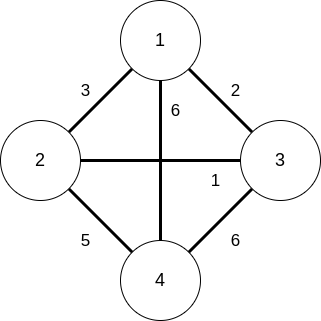
\includegraphics[scale=0.6]{img/graph.png}
	\end{center}
	\captionsetup{justification=centering}
	\caption{Взвешенный граф}
	\label{img:graph}
\end{figure}

По симметричности задача коммивояжера бывает:
\begin{itemize}
	\item симметричная - все пары ребер, соединяющие одни и те же вершины, имеют одинаковый вес (граф неориентированный);
	\item ассиметричная - вес пар ребер соединяющих одни и те же города, может различаться (ориентированный граф).
\end{itemize}

По замкнутости маршрута задача бывает: 
\begin{itemize}
	\item замкнутая - нахождение кратчайшего пути, проходящего через все вершины по одному разу с последующим возвратом в точку старта;
	\item незамкнутая — нахождение кратчайшего пути, проходящего через все вершины по одному разу и без обязательного возврата в исходную точку.
\end{itemize}

Далее будут рассмотрены алгоритмы решения симметричной замкнутой задачи коммивояжера.

Граф можно представить при помощи матрицы — таблицы, где строкам соответствуют города отправления, столбцам — города прибытия, а в ячейках указывается стоимость пути. Для графа на рисунке \ref{img:graph} матрица стоимостей будет следующая:
\clearpage
\begin{equation}
	A = \begin{pmatrix}
		0 & 3 & 2 & 6\\
		3 & 0 & 1 & 5\\
		2 & 1 & 0 & 6\\
		6 & 5 & 6 & 0\\
	\end{pmatrix}
\end{equation}

\section{Полный перебор}

Рассмотрим $n$ городов и матрицу расстояний между ними. Найдем самый короткий маршрут посещения всех городов ровно по одному разу, без возвращения в первый город:

\begin{itemize}
	\item число вариантов выбрать первый город равно $n$;
	\item число вариантов выбрать второй город равно $n - 1$;
	\item с каждым выбором следующего города число вариантов уменьшается на 1;
	\item число всех вариантов маршрутра равно $n!$;
	\item минимальный по сумме значений матрицы расстояний вариант маршрута - искомый.
\end{itemize}

В связи со сложностью $n!$ полный перебор вариантов занимает существенное время, а при большом количестве городов становится технически невозможным.

\section{Муравьиный алгоритм}

Идея муравьиного алгоритма \cite{ant} — моделирование поведения муравьев, связанное с их способностью быстро находить кратчайший путь и адаптироваться к изменяющимся условиям, находя новый кратчайший путь.

Муравьи действуют согласно правилам:
\begin{itemize}
	\item муравей запоминает посещенные города, причем каждый город может быть посещен только один раз. Обозначим через $J_{i,k}$ список городов, которые посетил муравей $k$, находящийся в городе $i$;
	\item муравей обладает видимостью $\eta_{ij}$ - эвристическим желанием посетить город $j$, если муравей находится в городе i, причем
\begin{equation}
	\label{d_func}
	\eta_{ij} = 1 / D_{ij},
\end{equation}
где $D_{ij}$ — стоимость пути из города $i$ в город $j$;
	\item муравей может улавливать след феромона - специального химического вещества. Число феромона на пути из города $i$ в город $j$ - $\tau_{ij}$.
\end{itemize}

Муравей выполняет следующую последовательность действий, пока не посетит все города:
\begin{itemize}
	\item выбирает следующий город назначения, основываясь на вероятностно-пропорциональном правиле \eqref{posib}, в котором учитываются видимость и число феромона:
\begin{equation}
	\label{posib}
	P_{ij, k} = \begin{cases}
		\frac{\tau_{ij}^\alpha\eta_{ij}^\beta}{\sum_{l=1}^m \tau^\alpha_{il}\eta^\beta_{il}}, \textrm{если город j необходимо посетить;} \\
		0, \textrm{иначе,}
	\end{cases}
\end{equation}
где $\alpha$ - параметр влияния феромона, $\beta$ - параметр влияния видимости пути, $\tau_{ij}$ - число феромона на ребре $(ij)$, $\eta_{ij}$ - эвристическое желание посетить город $j$, если муравей находится в городе $i$. Выбор города является вероятностным, данное правило определяет ширину зоны города $j$, в общую зону всех городов $J_{i,k}$ бросается случайное число, которое и определяет выбор муравья;
	\item муравей проходит путь $(ij)$ и оставляет на нем феромон.
\end{itemize}

Информация о числе феромона на пути используется другими муравьями для выбора пути. Те муравьи, которые случайно выберут кратчайший путь, будут быстрее его проходить, и за несколько передвижений он будет более обогащен феромоном. Cледующие муравьи будут предпочитать именно этот путь, продолжая обогащать его феромоном. 

После прохождения маршрутов всеми муравьями значение феромона на путях обновляется в соответствии со следующим правилом \eqref{update_phero_1}:

\begin{equation}
	\label{update_phero_1}
		\tau_{ij}(t+1) = (1-\rho)\tau_{ij}(t) + \Delta \tau_{ij},
\end{equation}
где $\rho$ - коэффициент испарения. Чтобы найденное локальное решение не было единственным, моделируется испарение феромона.

При этом
\begin{equation}
\label{update_phero_2}
 \Delta \tau_{ij} = \sum_{k=1}^m \tau_{ij, k},
\end{equation}
где $m$ - число муравьев,
\begin{equation}
	\label{update_phero_3}
		 \Delta\tau_{ij,k} = \begin{cases}
		Q/L_{k}, \textrm{если k-ый муравей прошел путь (i,j);} \\
		0, \textrm{иначе.}
	\end{cases}
\end{equation}

\section{Вывод}

Была изучена задача поиска оптимального маршрута, проходящего через все заданные вершины по одному разу. Были рассмотрены подходы к решению замкнутой симметричной задачи коммивояжера.

Программе, реализующей данные алгоритмы, на вход должна подаваться матрица стоимостей, которая задает взвешенный неориентированный граф. Выходными данными такой программы должны быть оптимальный маршрут, проходящий через все заданные вершины по одному разу с последующим возвратом в исходную точку, и его стоимость. Программа должна работать в рамках следующих ограничений: 

\begin{itemize}
	\item стоимости путей должны быть целыми числами;
	\item число городов должно быть больше 1;
	\item число дней должно быть больше 0;
	\item параметры муравьиного алгоритма должны быть вещественными числами, большими 0;
	\item матрица должна задавать неориентированный граф;
	\item должно быть выдано сообщение об ошибке при некорректном вводе параметров.
\end{itemize}

Пользователь должен иметь возможность выбора метода решения - полным перебором или муравьиным аогоритмом, и вывода результата на экран. Кроме того должна быть возможность проведения параметризации муравьиного алгоритма. Также должны быть реализованы сравнение алгоритмов по времени работы с выводом результатов на экран и получение графического представления результатов сравнения. Данные действия пользователь должен выполнять при помощи меню.